\section{Material test - water purification}
In this study the capacity of different materials (concrete, zeolite, goethite,
ion exchange and activated carbon) to adsorb metal ions in polluted water over
time was investigated. The material were added in SpinChem\textsuperscript{\textregistered}'s rotating
bed reactors (RBR). The materials were sieved (300-700~$\mu$m) and washed in
deionized water before studied. The concentration of metal ions (copper and
zinc) was measured by the analytic methods FAAS and ICP-OES.

The spectro analytical method atomic absorption spectroscopy (AAS) determines the concentration of metal ions by taking up the solution in a heated flame, where the metal ions excites and absorb light that passes the flame specific for the metal ion.\cite{ford} The analytical technique inductively coupled plasma optical emission spectroscopy (ICP-OES) is used for measuring of the concentrations of metal ions. It produce excited atoms and ions by using the inductively coupled plasma at wavelength that is specific for a certain type of metal ion. The analytical methods has different detection limits depending on machine and metal ions, but in general ICP-OES can detect lower levels of metal ion concentration than FAAS. ICP-OES can also analyze several metal ions at the same measurement while FAAS can only analyze one metal ion at a time\cite{boss}\cite{fassel}. 

To measure metal ion concentration 20~ml material was added to the RBR~S221 in the SpinChem\textsuperscript{\textregistered} reaction vessel V211 contained 200~ml polluted water and rotated at 700~rpm during two time intervals. Before starting the stirrer motor, a reference sample was taken and then samples were taken during a time interval. In the first set, all materials were investigated separately and samples were taken three times: 30 minutes, 60 minutes and 120 minutes. The experiment was repeated for concrete, zeolites and goethite with time interval: 10~seconds, 1~minute, 3~minutes, 7~minutes, 15~minutes and 30~minutes. All samples were taken with a syringe and filtered into falcon tubes. To each ml sample, 10 $\mu$l 7~M nitric acid was added in the falcon tubes and sent to FAAS analysis. 

After FAAS analyze, goethite was chosen for ICP-OES analyze to further investigate its capacity to adsorb metal ions in a larger scale. 50~ml material was added to the RBR~S331 in the reaction vessel V311 contained $1.2$~l polluted water and rotated at 700~rpm. Nine samples including the reference sample were taken with a time interval: 0~minutes, 10~seconds, 1~minutes, 3~minutes, 7~minutes, 15~minutes, 30~minutes, 1~hour and 2~hours. All samples were taken with a syringe and filtered into falcon tubes. To each ml sample, 10~\micro l 7~M nitric acid was added in the falcon tubes and analyzed with ICP-OES. 

To examine how the material (concrete and goethite) affect pH during the reaction 20~ml material was added to the RBR S221 in the reaction vessel V211 contained 200~ml polluted water and rotated at 700~rpm. pH was measured with litmus paper during a two hour period (see \cref{tab:ph}). 

\subsection{Results}
The capacity of the different materials (concrete, zeolite, goethite, ion exchange and activated carbon) to adsorb metal ions in polluted water over time was analysed. The metal ions, zinc and copper, were measured with the analytic methods FAAS and ICP-OES.

The FAAS analysis for the concentration of zinc ions showed that the concentration of zinc ions decreased for all materials after 30 minutes (see \cref{image00}). The same reference sample was used for all the materials. Goethite was the material that decreased most after 120~minutes, while concrete was the material with the lowest adsorption capacity. Between 30~minutes and 120~minutes, the concentration of zinc ions increased with concrete as material. The FAAS analysis for the concentration of copper ions showed that the concentration of copper ions decreased for all materials except zeolites after 120 minutes (see \cref{fig:image01}). Between 60~minutes and 120~minutes, the concentration of copper ions increased for concrete.

\begin{figure}[H]
    \centering
    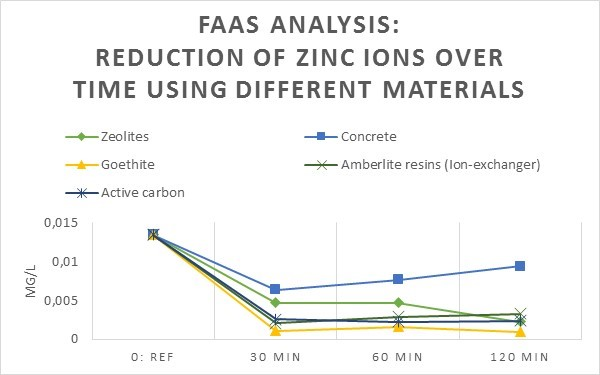
\includegraphics[width=0.7\textwidth]{image00}
    \caption{The concentrations of Zn$^{2+}$-ions in mg/l measured at four time
        points (0 min, 30 min, 60 min and 120 min) in five different materials
            (zeolites, goethite, active carbon, concrete and Amberlite resins)
            using the analytic method FAAS.}\label{fig:image00}
\end{figure}


\begin{figure}[H]
    \centering
    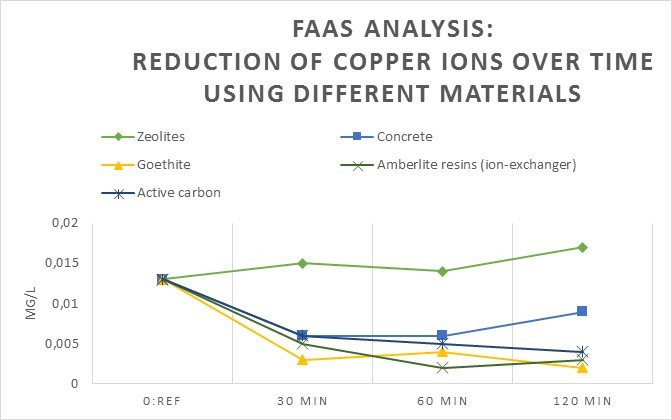
\includegraphics[width=0.7\textwidth]{image01}
    \caption{The concentrations of Cu$^{2+}$-ions in mg/l measured at four time
        points (0 min, 30 min, 60 min and 120 min) in five different materials
            (zeolites, goethite, active carbon, concrete and Amberlite resins)
            using FAAS analysis.}\label{fig:image01}
\end{figure}

The experiment was repeated for zeolites, concrete and goethite but with shorter time interval and more frequent sampling. The concentration of zinc ion was analysed with FAAS. After 10 seconds the concentration of zinc ions had increased for all materials (see \cref{fig:image02}). After 30 minutes, goethite was the material that had adsorb most zinc ions and with concrete as material, the concentration of zinc ions started to increase after 7 minutes.

\begin{figure}[H]
    \centering
    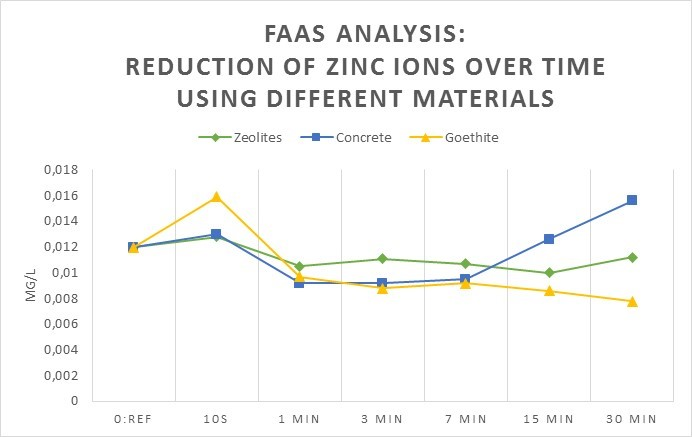
\includegraphics[width=0.7\textwidth]{image02}
    \caption{The concentrations of Zn$^{2+}$-ions in mg/l measured at seven time
        points (0 min, 10 s, 1 min, 3 min, 7 min, 15 min and 30 min) in three
            different materials (zeolites, concrete and goethite) using FAAS
            analysis.}\label{fig:image02}
\end{figure}

The result for the ICP-OES analysis with goethite showed that the concentration of copper ions decreased until 15~minutes and between 15~minutes and 120~minutes the concentration was stable at $0.02$~mg/l (\cref{fig:image03}). The result for the concentration of zinc ions with goethite displayed negative values but it seems to decrease until 3~minutes and then flatten out (\cref{fig:image04}).

\begin{figure}[H]
    \centering
    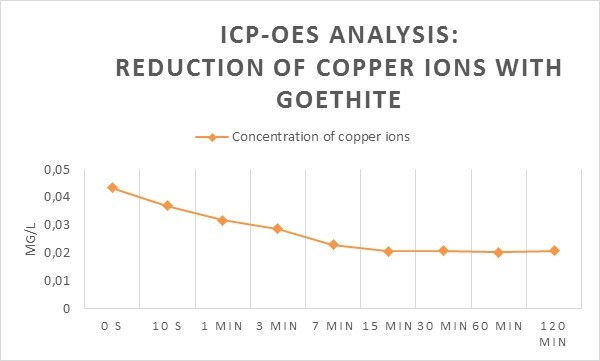
\includegraphics[width=0.7\textwidth]{image03}
    \caption{The concentration of Cu$^{2+}$-ions in mg/l measured at nine time
        points (0 s, 10 s, 1 min, 3 min, 7 min, 15 min, 30 min, 60 min and 120
                min) with goethite and analysed with ICP-OES.}\label{fig:image03}
\end{figure}


\begin{figure}[H]
    \centering
    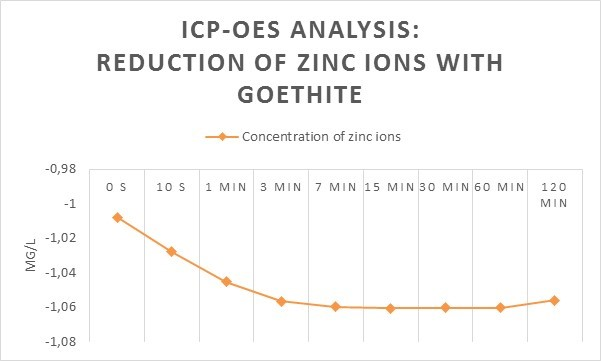
\includegraphics[width=0.7\textwidth]{image04}
    \caption{The concentration of Zn$^{2+}$-ions in mg/l measured at nine time
        points (0 s, 10 s, 1 min, 3 min, 7 min, 15 min, 30 min, 60 min and 120
                min) with goethite and analysed with ICP-OES.}\label{fig:image04}
\end{figure}

The result for pH measurements of concrete and goethite in polluted water containing metal ions showed to be stable at pH~5 for goethite during the whole time interval (\cref{tab:ph}). For concrete, the pH rose from 5 to 10 the first 5~minutes and then raised to 12 until 120~minutes. 

\begin{table}[H]
\centering
\caption{pH measurements with litmus paper of concrete and goethite at eight
    time points (0 min, 5 min, 10 min, 15min, 30 min, 60 min, 90 min and 120
            min) in polluted water containing metal ions.}
\label{tab:ph}
\begin{tabular}{lllllllll}
minutes         & 0 & 5 & 10 & 15 & 30 & 60 & 90 & 120 \\
pH for concrete & 5 & 10 & 11 & 11 & 12 & 12 & 12 & 12 \\
pH for goethite & 5 & 5 & 5 & 5 & 5 & 5 & 5 & 5
\end{tabular}
\end{table}

\subsection{Discussion}
A part of this project was to use SpinChem\textsuperscript{\textregistered}'s RBR and evaluate the capacity of different materials to adsorb metal ions in solution over time. The results from the FAAS analysis showed that all materials adsorb zinc ions after 120 minutes but had different capacities (\cref{fig:image00}). The concentration of zinc ions in the solution decreased more during the first 30 minutes and then the levels were quite stable. This could be due to that the materials became saturated and was not able to adsorb more zinc ions. The results also showed that concrete seemed to leak out zinc ions back to the solution after 30~minutes. This might be because the bond between zinc ions and concrete is weak and unstable or it favors other ions in the solution. The results for copper ions showed that all materials except zeolites were able to adsorb first 30 minutes (\cref{fig:image01}). As for the materials to adsorb zinc ions the result showed a similar pattern and after 30~minutes the concentration of copper ions were quite stable. This could be due to that the materials became saturated and was not able to adsorb more copper ions. It seems like the zeolite is not able to adsorb copper ions and might has greater affinity for other ions. 

Since the result for zinc ions showed a large decrease the first 30~minutes for all material we chose to repeat the experiment with zeolite, concrete and goethite during a shorter time interval and with more time points. The result was unexpected because the concentration of zinc ions were quite unchanged during the 30 minutes (\cref{fig:image02}). This could be due to that the standard that has to be prepared for FAAS analysis was too high comparing to our samples and therefore no conclusion can be made from this result. 

After FAAS analysis we decided to continue the study with goethite since it had the highest capacity to adsorb zinc ions and copper ions (\crefrange{fig:image00}{fig:image01}{fig:image02}). We repeated the experiment in larger scale ($1.2$~l) and chose to analyse with ICP-OES. The result showed that the reduction of copper ions in solution decreased most first 15~minutes and then the concentration were quite stable at $0.02$ (\cref{fig:image03}). Goethite seems to become saturated after 15~minutes and therefore not able to adsorb more copper ions. The result for the concentration of zinc ions in solution showed negative values of the concentration but displayed a similar pattern as for copper ions (\cref{fig:image04}). Goethite seems to be able to adsorb copper ions the first 7~minutes and then become saturated. The negatively values can be due to some error of measurement in ICP-OES machine. 
The pH measurements for concrete and goethite gave different results. For goethite, the pH level was stable around 5 during the whole time interval (\cref{tab:ph}). This might be due to that the material bind to other ions or release ions that does not affect the pH. The pH raised from 5 to 12 the whole time range and the large increase of the pH could be that concrete leaked out ions that affected the pH. The material could also bind hydrogen ions that affect the pH. 

In summary, goethite seems to have best capacity to adsorb zinc ions and copper ions comparing with the other materials and concrete seems to leak out the metal ions after time. Since the concentration of metal ions was extremely low in the solution, already in the beginning, the analysis methods seemed not to be good enough as analytical tool for the study and in future a more sensitive method should be used. 
